\documentclass[conference]{IEEEtran}

\usepackage{cite}
\usepackage{amsmath,amssymb,amsfonts}
\usepackage[T1]{fontenc}
\usepackage[utf8]{inputenc}
\usepackage[english]{babel} % Alterado para Inglês
\usepackage{algorithmic}
\usepackage{graphicx}
\usepackage{textcomp}
\usepackage{booktabs}
\usepackage{xcolor}
\usepackage{float}
\usepackage[section]{placeins}
\usepackage{dblfloatfix}
\usepackage{listings}
\usepackage[compatibility=false]{caption}
\usepackage{subcaption}

\def\BibTeX{{\rm B\kern-.05em{\sc i\kern-.025em b}\kern-.08em
    T\kern-.1667em\lower.7ex\hbox{E}\kern-.125emX}}

\renewcommand{\dbltopfraction}{0.9}
\renewcommand{\dblfloatpagefraction}{0.8}

\begin{document}

% MATLAB-style color definition
\definecolor{codegreen}{rgb}{0,0.6,0}
\definecolor{codegray}{rgb}{0.5,0.5,0.5}
\definecolor{codepurple}{rgb}{0.58,0,0.82}
\definecolor{backcolour}{rgb}{0.95,0.95,0.92}

\lstset{
    language=Matlab,
    backgroundcolor=\color{backcolour},   
    commentstyle=\color{codegreen},
    keywordstyle=\color{blue},
    numberstyle=\tiny\color{codegray},
    stringstyle=\color{codepurple},
    basicstyle=\ttfamily\scriptsize,
    breaklines=true,                  
    captionpos=b,                    
    keepspaces=true,                  
    numbers=left,                    
    numbersep=5pt,                  
    tabsize=2,
    frame=single,
    extendedchars=true,
    literate=
        {á}{{\'a}}1 {é}{{\'e}}1 {í}{{\'i}}1 {ó}{{\'o}}1 {ú}{{\'u}}1
        {Á}{{\'A}}1 {É}{{\'E}}1 {Í}{{\'I}}1 {Ó}{{\'O}}1 {Ú}{{\'U}}1
        {ã}{{\~a}}1 {õ}{{\~o}}1 {ç}{{\c{c}}}1 {Ã}{{\~A}}1 {Õ}{{\~O}}1
        {Ç}{{\c{C}}}1 {ê}{{\^e}}1 {Ê}{{\^E}}1 {à}{{\`a}}1 {À}{{\`A}}1
        {â}{{\^a}}1 {Â}{{\^A}}1 {î}{{\^i}}1 {Î}{{\^I}}1 {ô}{{\^o}}1 {Ô}{{\^O}}1
}

\title{Artificial Neural Networks \\ \large Assignment II - Regression with Neural Networks}

\author{\IEEEauthorblockN{1\textsuperscript{st} Leonardo Henriques}
\IEEEauthorblockA{\textit{University of Madeira, n°2120922} \\
}
\and
\IEEEauthorblockN{2\textsuperscript{nd} Leonardo Sousa}
\IEEEauthorblockA{\textit{University of Madeira, n°2123822} \\
}
}

\maketitle

\begin{abstract}
This study evaluates the performance of shallow neural networks in addressing two distinct environmental regression tasks: short-term wind speed forecasting and apparent temperature inference. A rigorous methodology was implemented, focusing on specialized pre-processing techniques such as trigonometric decomposition for cyclic features and logarithmic scaling for skewed distributions. Through a systematic grid search across various hidden layer sizes and activation functions, optimal architectures were identified and validated through 30 independent trials per configuration. The final models achieved high predictive precision, yielding a Mean Absolute Error (MAE) of $0.9669$ m/s for wind speed and $0.0432$ ºC for apparent temperature. These results demonstrate that the synergy between robust feature engineering and hyperparameter optimization enables shallow networks to achieve near-formulaic accuracy in complex meteorological forecasting problems.
\end{abstract}

\section{Introduction}
This report was developed within the scope of the \textit{Artificial Neural Networks} course. It details the training and evaluation of neural network models for two distinct regression tasks. For the \textit{windSpeed.csv} dataset, the objective is to predict wind speed one minute into the future based on historical data. Conversely, for the \textit{weatherHistory.csv} dataset, the goal is to infer the apparent temperature from various weather measurements.

\section{Methodology: \textit{windSpeed dataset}}
\subsection{Data Characterization}
The initial phase of this study involves exploratory data analysis and preprocessing to build a reliable predictive model for wind speed at Madeira International Airport. According to the assignment guidelines, the dataset comprises the following variables:
\begin{itemize}
    \item \textbf{Timestamp}: Date and time of the recording (yyyy-mm-dd hh:mm:ss format);
    \item \textbf{Wind Direction}: Wind direction (in degrees (º));
    \item \textbf{Wind Speed}: Wind velocity (in $m/s$);
\end{itemize}

\subsection{Data Cleaning and Pre-processing}
Upon loading the dataset, 1,048,575 observations were identified. The raw data contained two primary columns: \textit{CREATEDATE}, which aggregated the timestamp and wind direction, and \textit{DATA}, which recorded the wind speed. Initial preprocessing involved decomposing the \textit{CREATEDATE} column into distinct timestamp and direction variables, followed by renaming the features for clarity.

Subsequently, the dataset was inspected for inconsistencies, with a strong emphasis on temporal continuity—a critical requirement for time-series forecasting. While no duplicate records were found, minor missing values were detected (two for wind speed and one for wind direction). Given the brief duration of these gaps (a maximum of seven seconds, excluding a massive gap in February, as illustrated in Figure 1), linear interpolation was applied. Finally, the dataset was segmented into continuous blocks wherever chronological interruptions exceeded 70 seconds. This strategy divided the data into two primary contiguous blocks, effectively isolating the large data gap observed in February.

\begin{figure}[H]
    \centering
    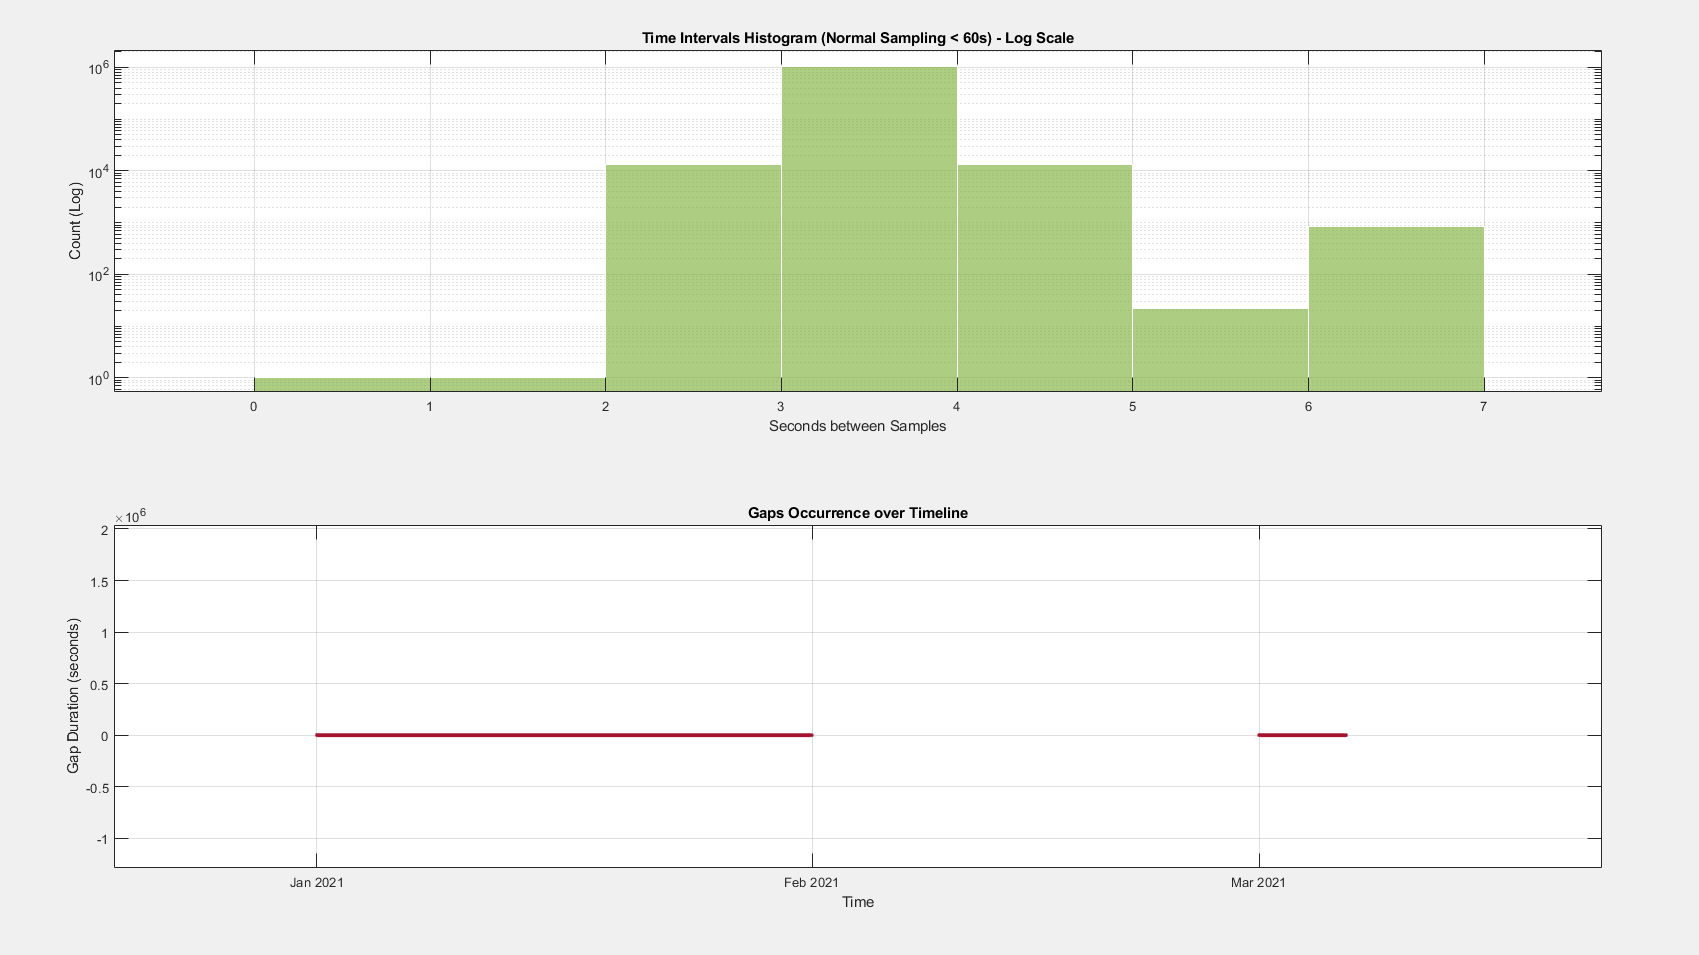
\includegraphics[width=\columnwidth]{imagens_windspeed/time_interval_and_gaps.png}
    \caption{Time intervals and missing gaps in the windSpeed dataset.}
\end{figure}

\subsection{Feature Engineering and Selection}





To enhance model performance and capture underlying temporal and physical dynamics, the following features were engineered:

\begin{itemize}
    \item \textbf{Cyclic Transformation of Wind Direction:} Sine and cosine functions were applied to the wind direction to preserve its circular nature. This geometric encoding prevents the neural network from incorrectly interpreting the transition between 359º and 1º as a massive 358º numerical difference.
\begin{lstlisting}[language=Matlab, caption={Trigonometric encoding of the wind direction},captionpos=t] 
theta_rad = deg2rad(data.WindDirection);
data.Dir_Sin = sin(theta_rad);
data.Dir_Cos = cos(theta_rad);
\end{lstlisting}   
    \item \textbf{Temporal Encoding:} The time of day was converted into a continuous decimal format and subsequently transformed into periodic sine and cosine components. This ensures the model recognizes the cyclic proximity of late-night and early-morning hours.
\begin{lstlisting}[language=Matlab, caption={Trigonometric encoding of the timestamp},captionpos=t] 
horas_decimais = hour(data.Time) + minute(data.Time)/60 + second(data.Time)/3600;
data.Hour_Sin = sin(2 * pi * horas_decimais / 24);
data.Hour_Cos = cos(2 * pi * horas_decimais / 24);
\end{lstlisting}   
    \item \textbf{Wind Acceleration:} Derived using the finite difference between the current and previous wind speed measurements. Exception handling was implemented at the beginning of each block to avoid invalid cross-block calculations.
\begin{lstlisting}[language=Matlab, caption={Wind Acceleration},captionpos=t] 
data.Wind_Acc = [0; diff(data.WindSpeed)];
idx_block_starts = [1; find(diff(data.BlockID) > 0) + 1];
data.Wind_Acc(idx_block_starts) = 0;
\end{lstlisting}   
\end{itemize}

Finally, the target variable (\textit{Target\_WindSpeed}) was constructed. For each observation $t$, a look-ahead search was performed to locate the exact future wind speed at $t + 60$ seconds.

\begin{lstlisting}[language=Matlab, caption={Look-ahead loop to find the future values of wind speed}, captionpos=t]
time_numeric = cumsum(data.TimeDiff);
speeds = data.WindSpeed;
targets = NaN(size(speeds));
block_ids = data.BlockID;

block_starts = [1; find(diff(block_ids) > 0) + 1];
block_ends = [block_starts(2:end) - 1; length(block_ids)];

for b = 1:length(block_starts)
    start_idx = block_starts(b);
    end_idx = block_ends(b);
    if end_idx > start_idx
        j = start_idx;
        for i = start_idx:end_idx
            while j <= end_idx && (time_numeric(j) - time_numeric(i)) < 60
                j = j + 1;
            end
            if j <= end_idx
                targets(i) = speeds(j);
            end
        end
    end
end

\end{lstlisting}

We also applied a logarithmic transformation to the wind speed data, as it exhibited a right-skewed distribution. This allowed us to significantly reduce the number of outliers and stabilize model convergence, as the models were less affected by extreme wind speed values, leading to a smoother optimization process.

\begin{figure}[H]
    \centering
    \begin{subfigure}{\columnwidth}
        \centering
        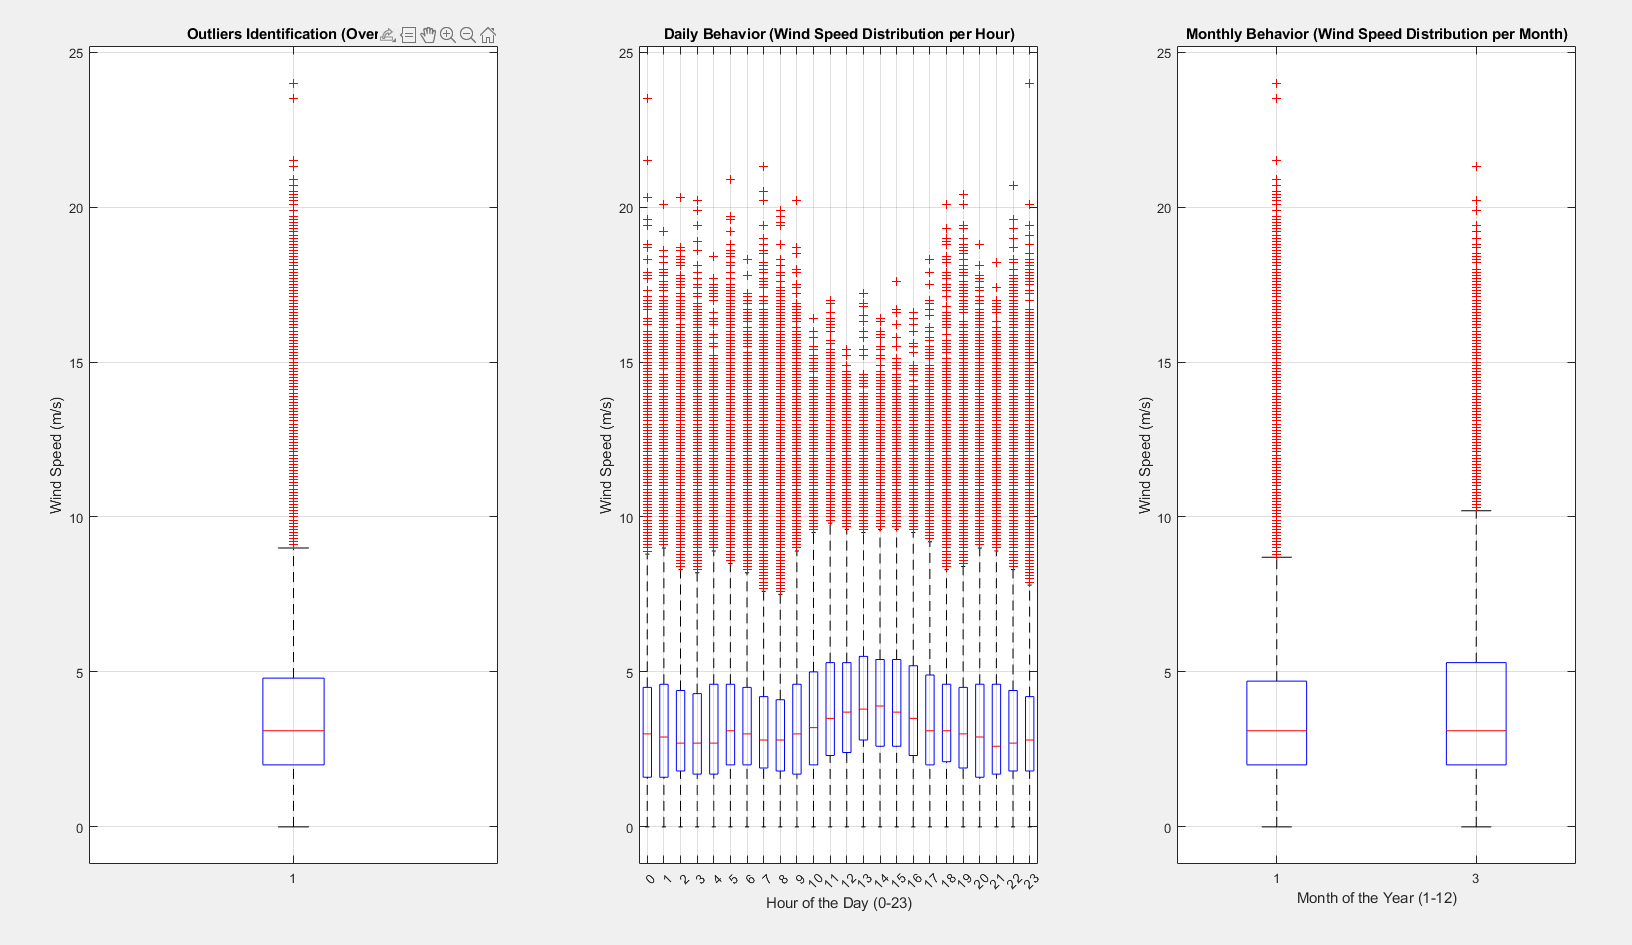
\includegraphics[width=\linewidth]{imagens_windspeed/boxplots do vento.png}
        \caption{Before log1 transformation.}
        \label{fig:wind_before}
    \end{subfigure}
    \vspace{0.3cm}
    \begin{subfigure}{\columnwidth}
        \centering
        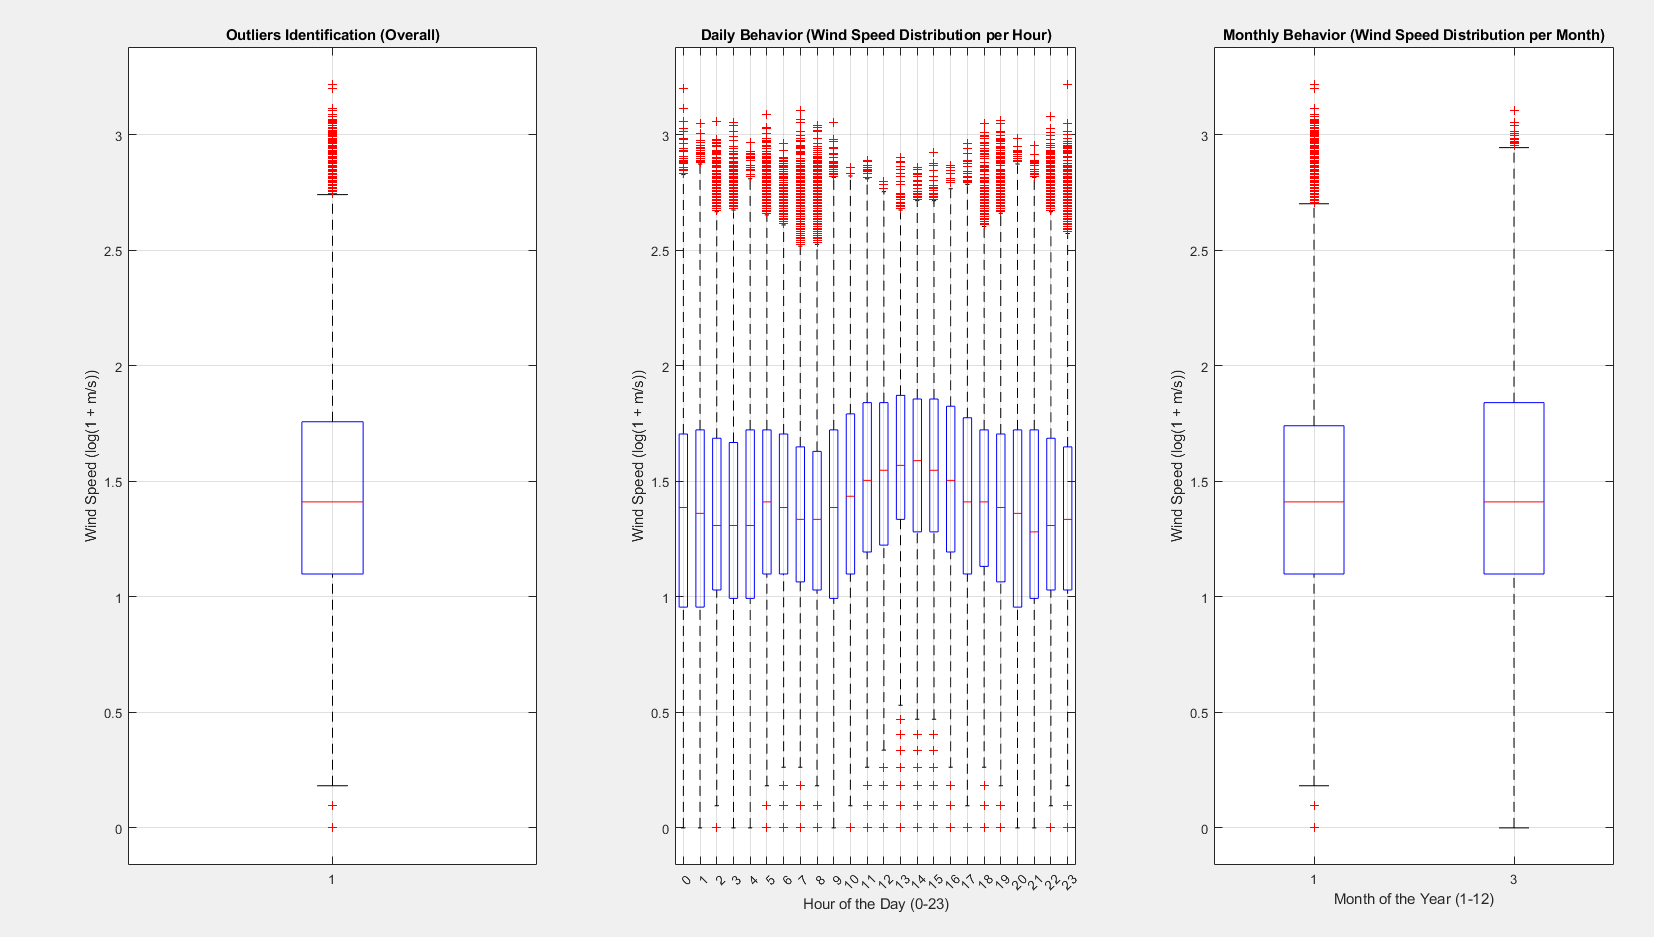
\includegraphics[width=\linewidth]{imagens_windspeed/boxplots log(windspeed).png}
        \caption{After log1 transformation.}
        \label{fig:wind_after}
    \end{subfigure}
    \caption{Comparison of wind speed distribution before and after log1 transformation.}
    \label{fig:wind_comparison}
\end{figure}

To further visualize the impact of these pre-processing steps, Figure \ref{fig:temporal_evolution} illustrates the temporal behavior of the wind speed (after logarithmic scaling), the wind direction, and the engineered wind acceleration.

\begin{figure}[H]
    \centering
    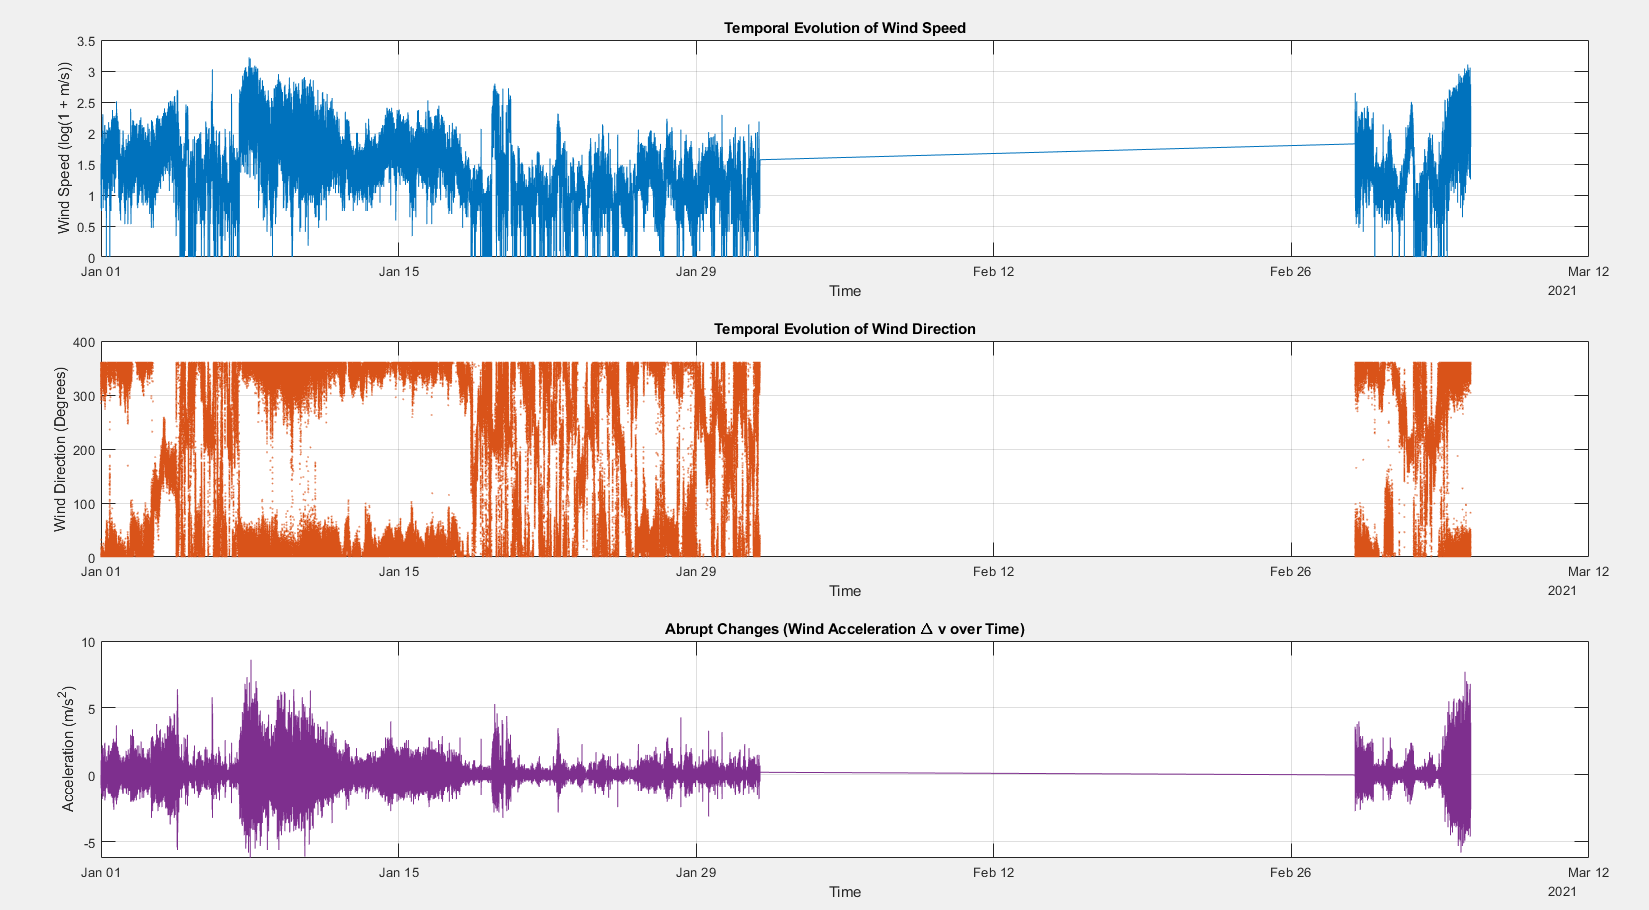
\includegraphics[width=\columnwidth]{imagens_windspeed/evolução temporal apos log.png}
    \caption{Temporal evolution of the log-transformed wind speed, wind direction, and acceleration.}
    \label{fig:temporal_evolution}
\end{figure}

The temporal evolution of the processed features confirms the effectiveness of the transformations. The top panel shows the wind speed after the $\log(1+v)$ scaling, which compresses the range of values and stabilizes the variance, making the series more suitable for gradient-based optimization. The large data gap in February is clearly visible, justifying the block-based segmentation strategy. The bottom panel displays the wind acceleration, which captures the instantaneous rate of change and provides the network with a representation of the physical momentum, a key factor in improving short-term predictive accuracy.

The final curated dataset comprises the original inputs, the newly engineered features, and the target variable. Following this phase, a final correlation analysis was conducted. 

\begin{figure}[H]
    \centering
    \begin{subfigure}{\columnwidth}
        \centering
        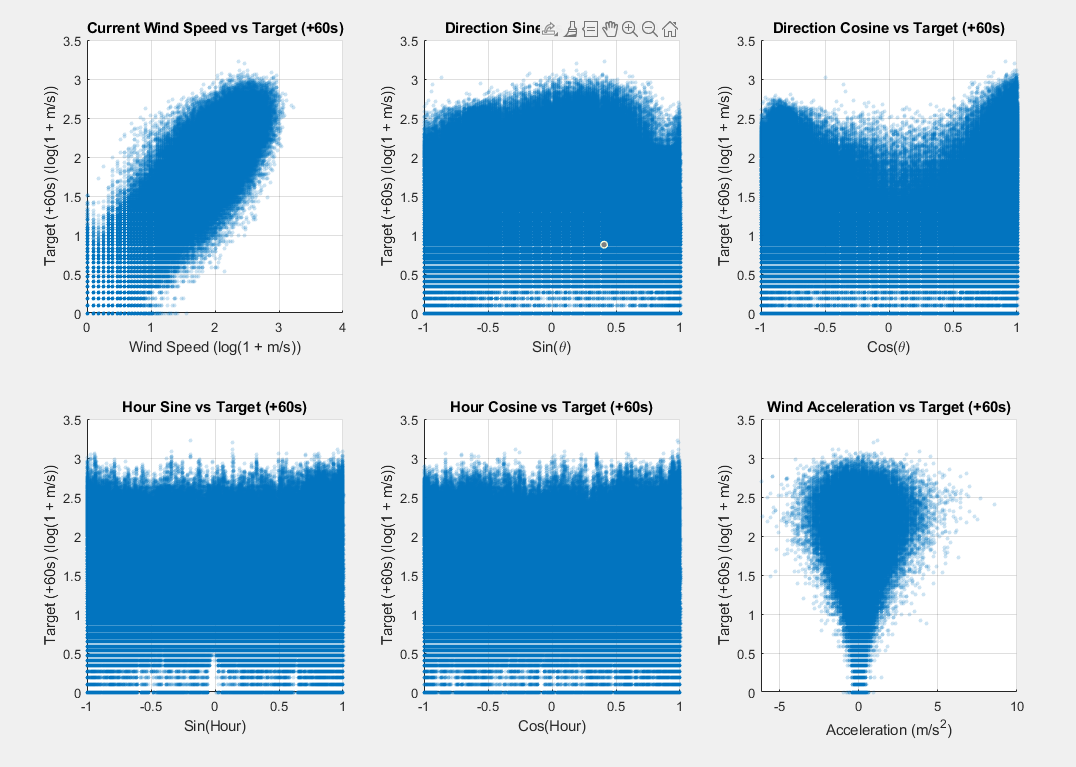
\includegraphics[width=\linewidth]{imagens_windspeed/scatter log wind.png}
        \caption{Scatter plots.}
    \end{subfigure}
    \vspace{0.3cm}
    \begin{subfigure}{\columnwidth}
        \centering
        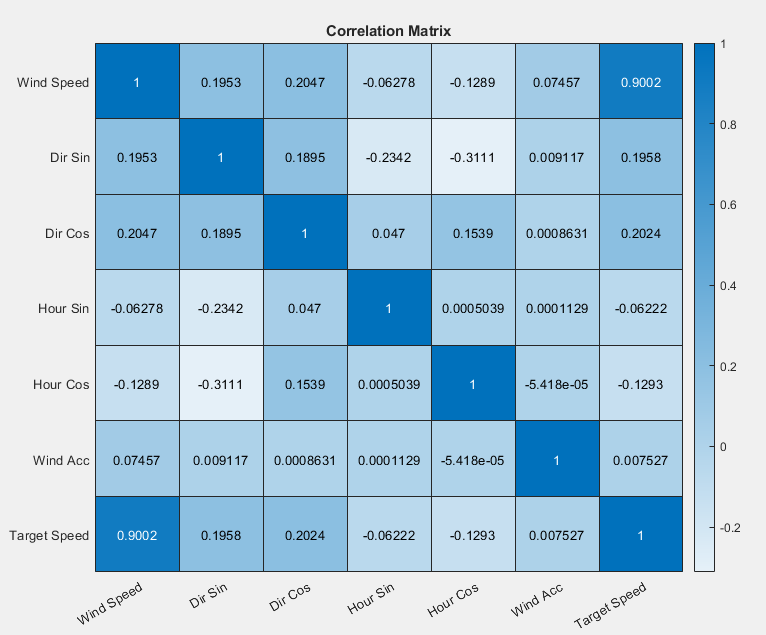
\includegraphics[width=\linewidth]{imagens_windspeed/corr_poslog.png}
        \caption{Correlation matrix.}
    \end{subfigure}
    \caption{Feature analysis.}
    \label{fig:feature_analysis}
\end{figure}


As shown in Figure 3, the engineered features exhibit low linear correlation with the target variable, with the exception of the current wind speed, which is expected given the target is a temporal displacement of this feature. However, this lack of linear correlation does not hinder the predictive capability of the model, as neural networks excel at extracting complex, non-linear relationships from such multi-dimensional data.


Based on the exploratory data analysis and the feature engineering process, the final subset of input features selected to train the predictive model consists of the following six variables:

\begin{itemize}
    \item \textbf{WindSpeed} (log-transformed): The current wind velocity, acting as the primary baseline for the short-term forecast.
    \item \textbf{Dir\_Sin and Dir\_Cos}: The decomposed trigonometric components of the wind direction, providing a continuous spatial orientation without the 360º-to-0º discontinuity.
    \item \textbf{Hour\_Sin and Hour\_Cos}: The cyclical encoding of the timestamp, enabling the network to learn diurnal patterns driven by solar heating.
    \item \textbf{Wind\_Acc}: The instantaneous rate of change in wind speed, informing the model whether the wind momentum is currently in an upward or downward trend.
\end{itemize}

Original variables such as the raw timestamp, block identifiers, and the linear wind direction in degrees were deliberately discarded from the final dataset. Removing these features prevents redundancy, eliminates spatial discontinuities, and mitigates the risk of the neural network learning spurious artifacts. 

This compact and highly informative feature set aligns with best practices for shallow neural network training, ensuring a balanced, scaled, and physically sound input space capable of capturing both the momentum and the cyclical patterns of the wind.


\section{Methodology: \textit{weatherHistory dataset}}

\subsection{Data Characterization}

The data set consists of 96453 values and 8 features. Our objective is to analyze them and, through data cleaning and feature engineering, obtain a data set to train a neural network capable of predicting the apparent temperature, it being our variable target.

The features are as follows:

\begin{itemize}
    \item \textbf{Temperature\_C}: The temperature at a given moment in Celsius (Cº);
    \item \textbf{Apparent\_Temperature\_C}: The equivalent perceived by humans, also in Celsius (Cº);
    \item \textbf{Humidity}: The humidity percentage of said moment, its values are presented between 0 and 1;
    \item \textbf{Wind\_Speed\_km\_h\_}: The wind's speed in kilometers per hour (km/h);
    \item \textbf{WindBearing\_degrees\_}: The direction of which the wind is blowing from in degrees;
    \item \textbf{Visibility\_km\_}: The maximum distance that an object can be perceived in the current weather in kilometers (km);
    \item \textbf{Cloud\_Cover}: If there are clouds covering the sky or not, with one representing a fully clouded sky and zero representing clear skies;
    \item \textbf{Pressure\_millibars\_}: The atmospheric pressure measured in millibars (mbar).

\end{itemize}

It is important to note that in the data set the feature Cloud Cover is presented as \textit{LoudCover}, as this is most likely a error, and as I found no use for the feature and later removed it. I decided to not change it's name in the data set and rename it in the report. 

\subsection{Data Cleaning and Pre-processing}

Firstly we analysed the amount of zeros and values missing. There were no values missing in the data set. Although there were zeros in all the features.

After analysing the distribution of the data, the box plots, the correlation matrix and scatterplot we can notice that our data set has errors in these last analysis. There is a small amount of zeros in the distribution of the feature related to the atmospheric pressure and humidity. Which can't be possible in natural environments, which means that they are more likely to be errors. Furthermore the feature Cloud Coverage possesses mostly zero values Which explains why they appear as a \textit{NaN} in the Correlation Matrix.

\begin{figure}[H]
    \centering
    \includegraphics[width=\columnwidth]{imagens_weatherHistory/Distribuição das Features Iniciais.jpeg}
    \caption{Distribution of the Features.}
\end{figure}


\begin{figure}[H]
    \centering
    
\includegraphics[width=\columnwidth]{imagens_weatherHistory/Boxplot de Features Iniciais.jpeg}
    \caption{Boxplot of the Features.}
\end{figure}


\begin{figure}[H]
    \centering
    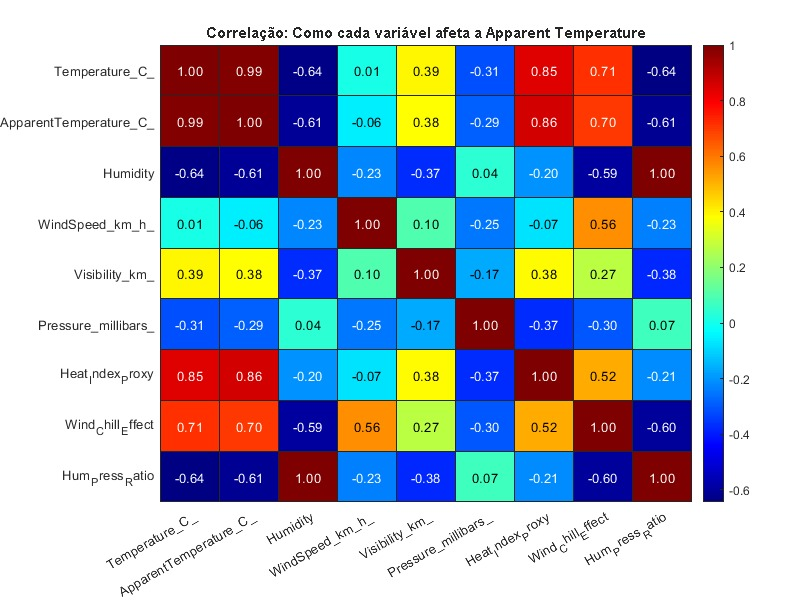
\includegraphics[width=\columnwidth]{imagens_weatherHistory/Matriz de Correlação de Features Finais.jpeg}
    \caption{Correlation Matrix of the features.}
\end{figure}

As observed Correlation Matrix we can tell that Temperature and Humidity have a very High correlation to our target variable, \textit{Apparent\_Temperature\_C\_}, Visibility also has some correlation to it too.

Given all this information I decided to clean the zeros in Humidity and Pressure and also remove the feature Cloud Cover.

To clean the data I decided to use Linear Interpolation to correct the zeros and deleted any missing value the interpolation didn't manage to correct.

\subsection{Feature Engineering and Selection}

For the feature engineering I decided to think about what could possibly affect the temperature. Additionally in order to try and make Wind Direction possibly relevant, and to help with the neural network training, I decided to remove it and decompose it in both Sine and Cosine, although I still had doubts it would provide something useful. With this in mind I created:

\begin{itemize}
    \item \textbf{Wind\_Sin and Wind\_Cos}: The decomposition of the feature Wind Direction in degrees;

    \begin{lstlisting}[language=Matlab, caption={Wind Direction Decomposition},captionpos=t] 
    data.Wind_Sin = sin(deg2rad(data.WindBearing_degrees_));
    data.Wind_Cos = cos(deg2rad(data.WindBearing_degrees_));
    \end{lstlisting}  
    
    \item \textbf{Heat\_Index\_Proxy}: Obtained after multiplying Temperature and Humidity. It represents a simpler substitution of the more complex calculations in Heat Index;

    \begin{lstlisting}[language=Matlab, caption={Heat\_Index\_Proxy},captionpos=t] 
    data.Heat_Index_Proxy = data.Temperature_C_ .* data.Humidity;
    \end{lstlisting}  
    
    \item \textbf{Wind\_Chill\_Effect}: By multiplying Wind Speed and Temperature we should have something that represents the wind's effect in the temperature.

    \begin{lstlisting}[language=Matlab, caption={Wind\_Chill\_Effect},captionpos=t] 
    data.Wind_Chill_Effect = data.WindSpeed_km_h_ .* data.Temperature_C_;
    \end{lstlisting}  
    
    \item \textbf{Hum\_Press\_Ratio}: We get it by multiplying Humidity with Pressure, it represents the density and stability of air, since an higher pressure and humidity means a higher retention of heat.

    \begin{lstlisting}[language=Matlab, caption={Hum\_Press\_Ratio},captionpos=t] 
    data.Hum_Press_Ratio = data.Humidity .* data.Pressure_millibars_;
    \end{lstlisting}  
    
\end{itemize} 

\begin{figure}[H]
    \centering
    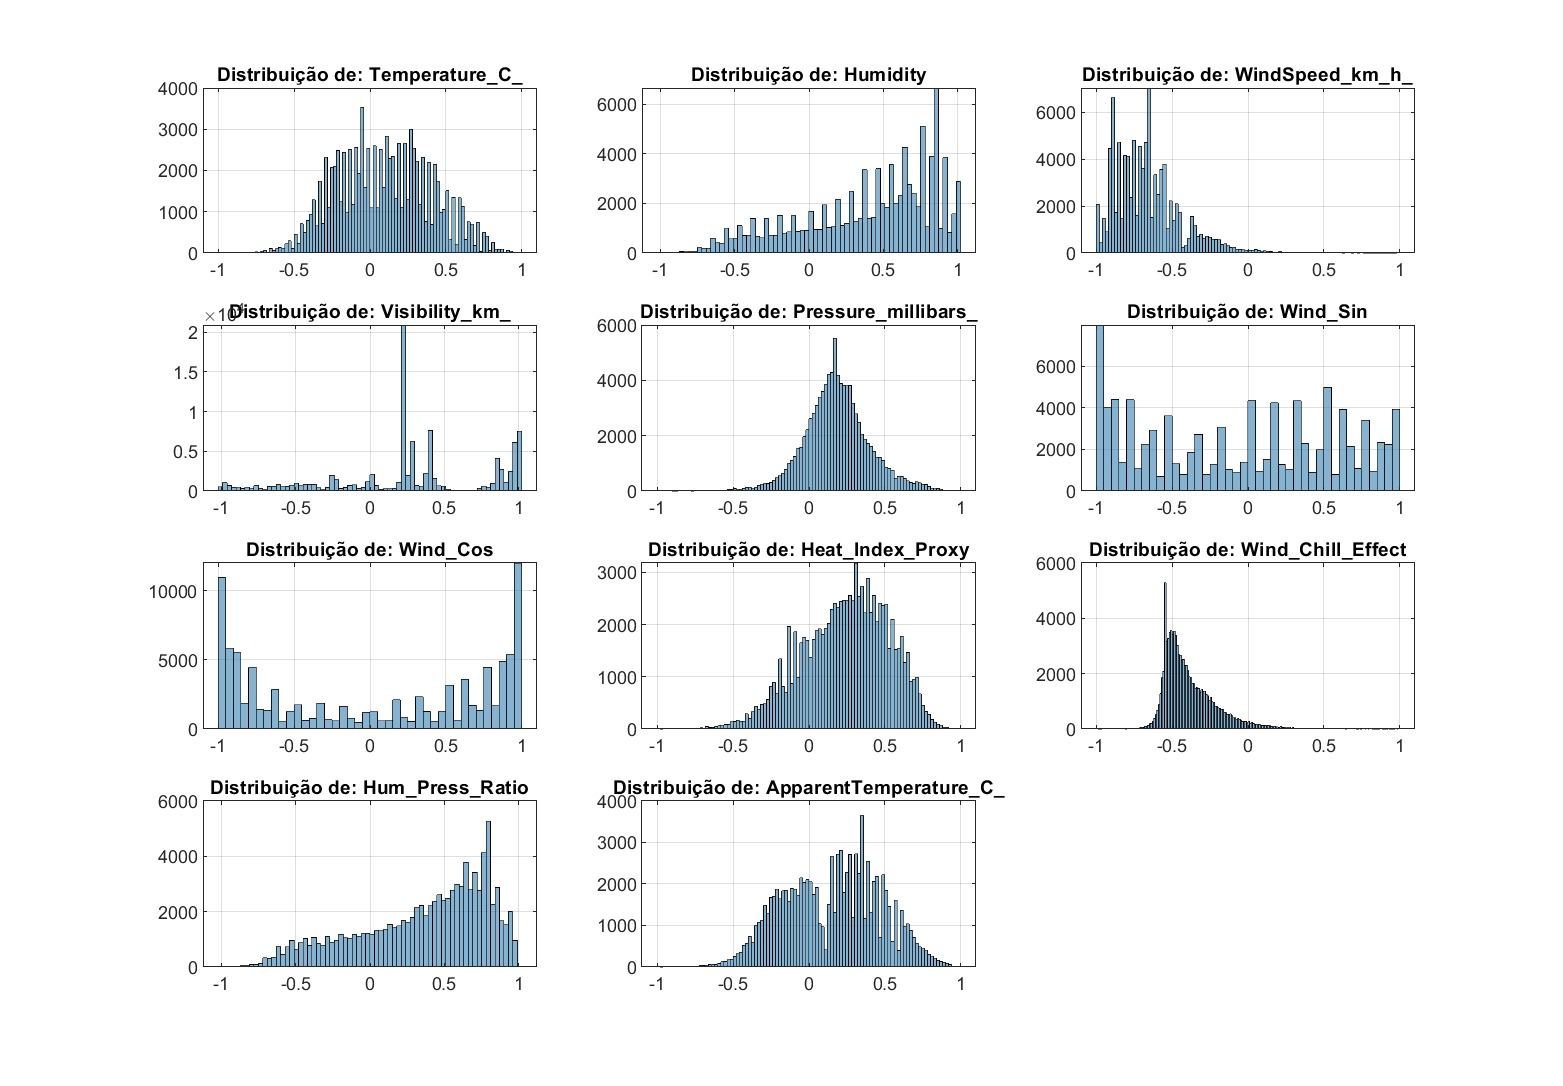
\includegraphics[width=\columnwidth]{imagens_weatherHistory/Distribuições depois de Feature Engineering.jpeg}
    \caption{Distribution of the Features after Feature Engineering.}
\end{figure}


\begin{figure}[H]
    \centering
    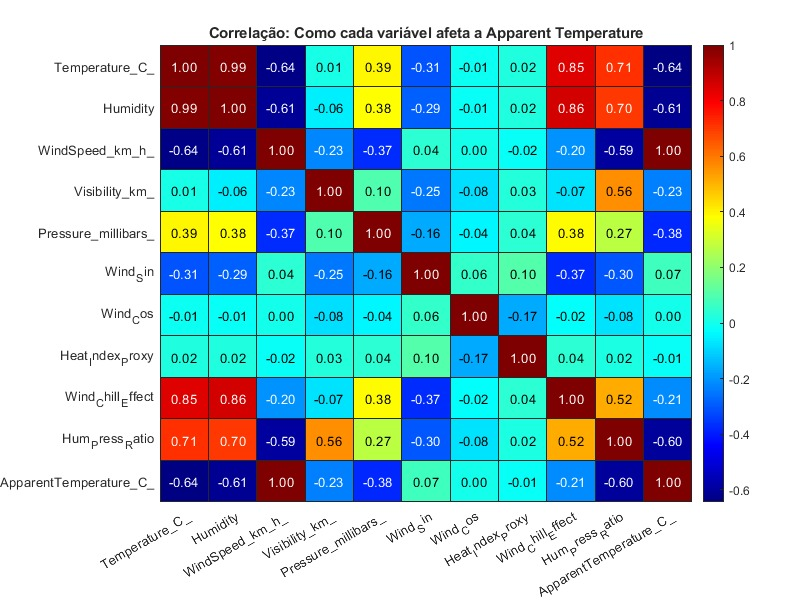
\includegraphics[width=\columnwidth]{imagens_weatherHistory/Matriz de Correlação depois de Feature Engineering.jpeg}
    \caption{Correlation Matrix after feature engineering.}
\end{figure}

After analysing with the same graphs previously mentioned I arrived at the conclusion that the correlation between the target variable and the decomposition of Wind Direction does not justify their creation and as such I deleted them.
Ending with the following Features:

\begin{itemize}
    \item \textbf{Temperature\_C\_}: Current air temperature;
    \item \textbf{Apparent\_Temperature\_C\_}: Target variable (perceived temperature);
    \item \textbf{Humidity}: Relative humidity;
    \item \textbf{WindSpeed\_km\_}: Wind velocity;
    \item \textbf{Visibility\_km\_}: Visual distance;
    \item \textbf{Pressure\_millibars\_}: Atmospheric pressure;
    \item \textbf{Heat\_Index\_Proxy}: Combined temperature and humidity;
    \item \textbf{Wind\_Chill\_Effect}: Combined wind and temperature;
    \item \textbf{Hum\_Press\_Ratio}: Combined humidity and pressure.
\end{itemize}

\begin{figure}[H]
    \centering
    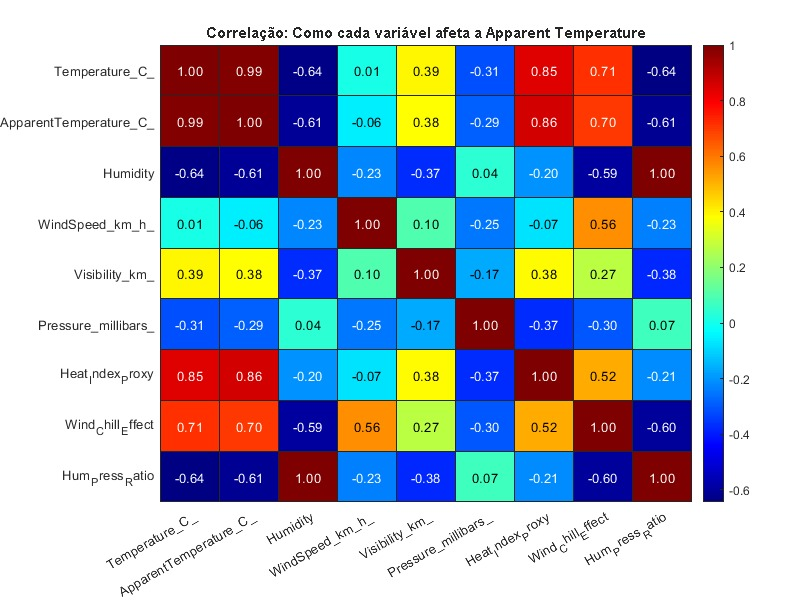
\includegraphics[width=\columnwidth]{imagens_weatherHistory/Matriz de Correlação de Features Finais.jpeg}
    \caption{Correlation Matrix of the Final Features.}
\end{figure}

\subsection{Data Partitioning}
Since the weather dataset observations represent independent atmospheric measurements rather than a sequential forecasting problem, a randomized data partitioning strategy was adopted. The dataset was randomly shuffled and split into 90\% for training and validation (86,807 samples), and 10\% for the final held-out test set (9,646 samples). This randomized approach ensures that both sets contain a representative distribution of various weather conditions, mitigating any seasonal or chronological bias present in the raw data order.


\section{Models training}
\subsection{Network Architecture and Hyperparameters}
For both regression tasks, a shallow feedforward neural network architecture, specifically MATLAB's \texttt{fitnet}, was employed with a single hidden layer. While forecasting wind speed is inherently a dynamic time-series problem---typically requiring recurrent architectures such as NARNet or NARXNet---our data preparation strategy allowed for a simpler and more efficient approach. By explicitly engineering the target variable (locating the wind speed exactly one minute into the future and aligning it with the current inputs), the temporal shift was inherently embedded into the dataset. This transformation effectively reduced the dynamic forecasting task to a standard static multivariate regression problem, fully justifying the use of a standard feedforward architecture for both the wind speed and the weather station datasets.
To determine the optimal network configuration, a grid search was conducted over two primary hyperparameters: the number of hidden neurons and the activation function. The hidden layer size was varied across four configurations (5, 10, 15, and 20 neurons) to evaluate the optimal balance between model capacity and generalization, aiming to prevent both underfitting and overfitting.
Regarding the hidden layer's activation function, two distinct mathematical approaches were evaluated: the Hyperbolic Tangent Sigmoid (\texttt{tansig}) and the Positive Linear (\texttt{poslin}, equivalent to ReLU). The \texttt{tansig} function was selected because its smooth, zero-centered nature (outputting values between -1 and 1) is traditionally highly effective for capturing complex, non-linear relationships in normalized regression tasks. Conversely, the \texttt{poslin} function was introduced to assess its sparsity and non-saturating properties for positive values, which helps mitigate the vanishing gradient problem and is particularly well-suited for unbounded physical measurements.


\subsection{Training Strategy and Approach}
To ensure robust and statistically significant results, the training strategy was designed in accordance with the Central Limit Theorem. The hyperparameter grid search yielded 8 distinct configuration points, representing all combinations of the selected neuron counts and activation functions. For each configuration, the neural network was initialized and trained 30 independent times. This comprehensive evaluation, totaling 240 training runs per dataset, allowed for a rigorous assessment of model convergence and stability, mitigating the variance inherent to stochastic weight initialization.
During the optimization phase, models for both datasets were trained using the Mean Squared Error (MSE) as the primary performance function. MSE was chosen to effectively penalize larger prediction errors during the weight update process, which was driven by the Levenberg-Marquardt backpropagation algorithm (\texttt{trainlm}). Once the optimal combination of hyperparameters was identified, based on the lowest average validation MSE, a final, definitive model was trained. To provide a highly interpretable assessment of the model's real-world accuracy, this final network was evaluated against an isolated, completely unseen test dataset using the Mean Absolute Error (MAE) metric. This final evaluation ensures that the reported performance reflects the absolute physical deviation in the target variables' native units.


\section{Results}
\subsection{Performance and Metrics (\textit{windSpeed dataset})}
The empirical results of the hyperparameter grid search for the wind speed forecasting task are summarized in Table \ref{tab:wind_optimization}. Following the training of 30 independent models for each of the 8 configurations, the \texttt{poslin} (ReLU) activation function consistently demonstrated superior performance compared to \texttt{tansig}, particularly as the network complexity increased.

\begin{table}[!t]
    \centering
    \caption{Neural Network Optimization Results for windSpeed dataset}
    \label{tab:wind_optimization}
    \vspace{1em}
    \begin{tabular}{cccc}
        \toprule
        \textbf{Neurons} & \textbf{Activation} & \textbf{Mean Val MSE} & \textbf{Variance Val MSE} \\
        \midrule
        5  & "tansig" & 0.041729 & $3.2583 \times 10^{-8}$ \\
        5  & "poslin" & 0.041814 & $1.4747 \times 10^{-7}$ \\
        10 & "tansig" & 0.041574 & $4.4508 \times 10^{-8}$ \\
        10 & "poslin" & 0.041441 & $4.1427 \times 10^{-8}$ \\
        15 & "tansig" & 0.041476 & $3.7216 \times 10^{-8}$ \\
        \textbf{15} & \textbf{"poslin"} & \textbf{0.041365} & \boldmath{$3.2485 \times 10^{-8}$} \\
        20 & "tansig" & 0.041599 & $2.9701 \times 10^{-8}$ \\
        20 & "poslin" & 0.041365 & $1.8877 \times 10^{-8}$ \\
        \bottomrule
    \end{tabular}
    \par\vspace{1ex}
    \small \textbf{Note:} Highlighted row indicates the optimal configuration based on the trade-off between error and model parsimony.
\end{table}

\begin{figure}[H]
    \centering
    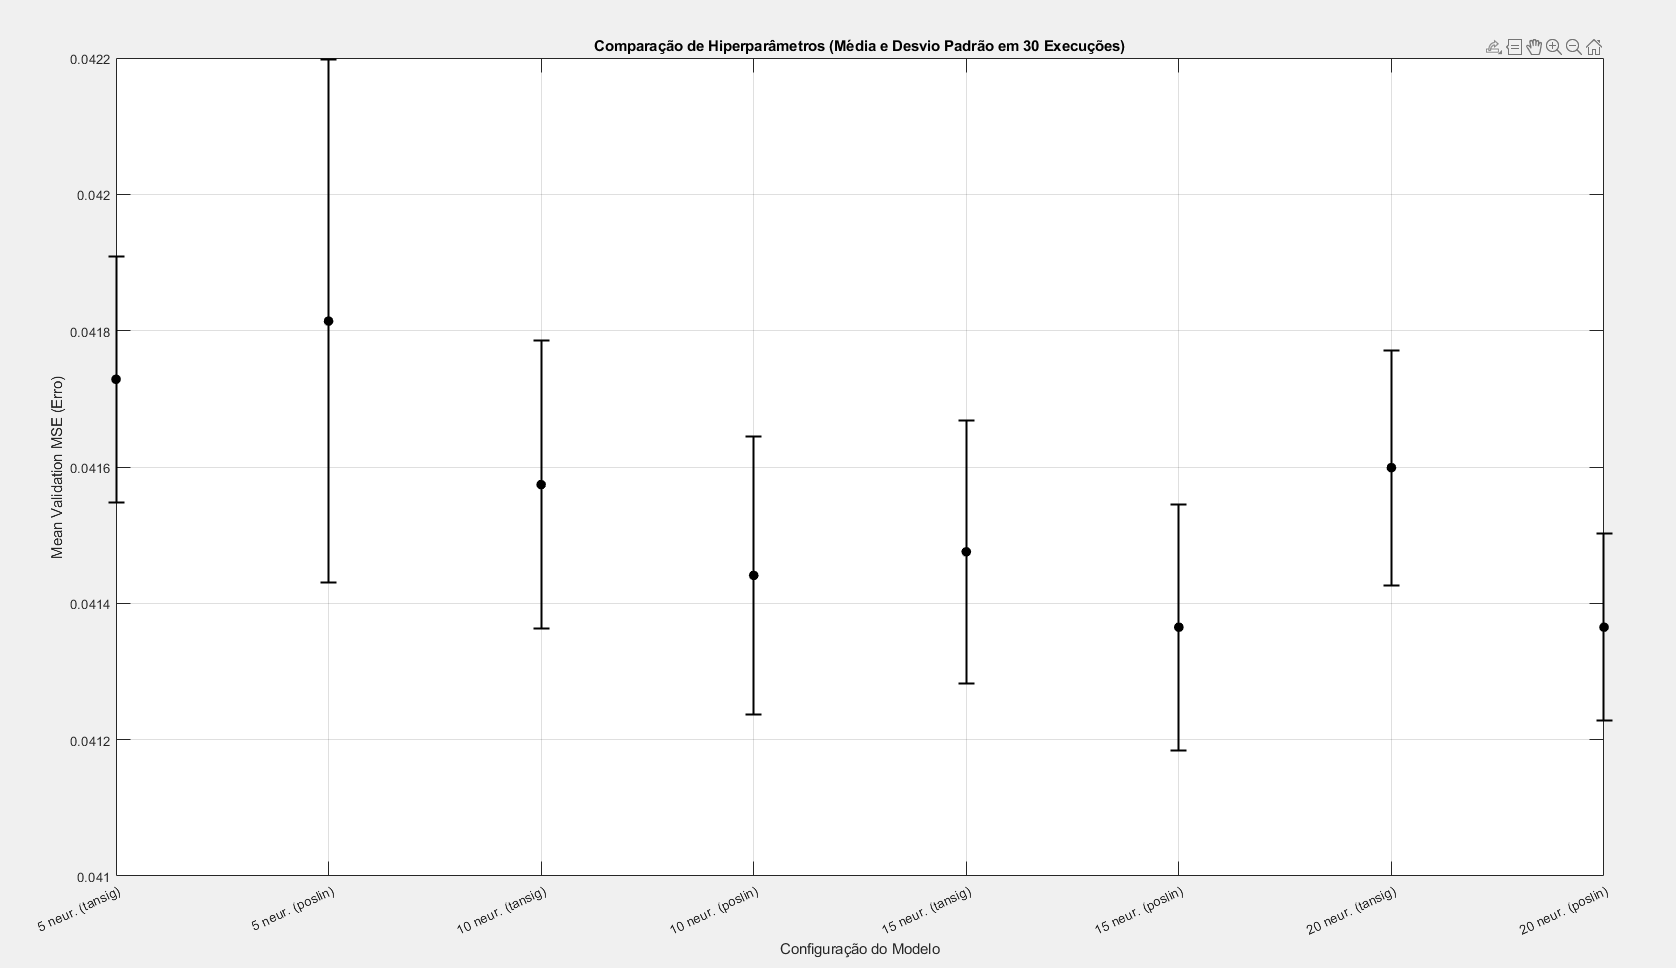
\includegraphics[width=\columnwidth]{imagens_windspeed/comp_diff_configs_aposlog.png}
    \caption{Comparative analysis of mean and standard deviation of MSE across different configurations.}
    \label{fig:wind_comparison_configs}
\end{figure}

As illustrated in Figure \ref{fig:wind_comparison_configs}, the \texttt{poslin} models generally achieved lower error rates and exhibited greater stability across different neuron counts. The configuration with 15 neurons and the \texttt{poslin} activation function was selected as the optimal architecture. While the 20-neuron \texttt{poslin} model yielded a similar mean error, the 15-neuron variant offers a more efficient balance between predictive power and computational simplicity, effectively mitigating the risk of overfitting.


Following the selection of the optimal configuration, a final definitive model was trained on the full training set and validated. The optimization curve, depicted in Figure \ref{fig:wind_training_curve}, demonstrates a smooth and consistent convergence of both training and validation errors, indicating a robust learning process and high generalization potential.

\begin{figure}[H]
    \centering
    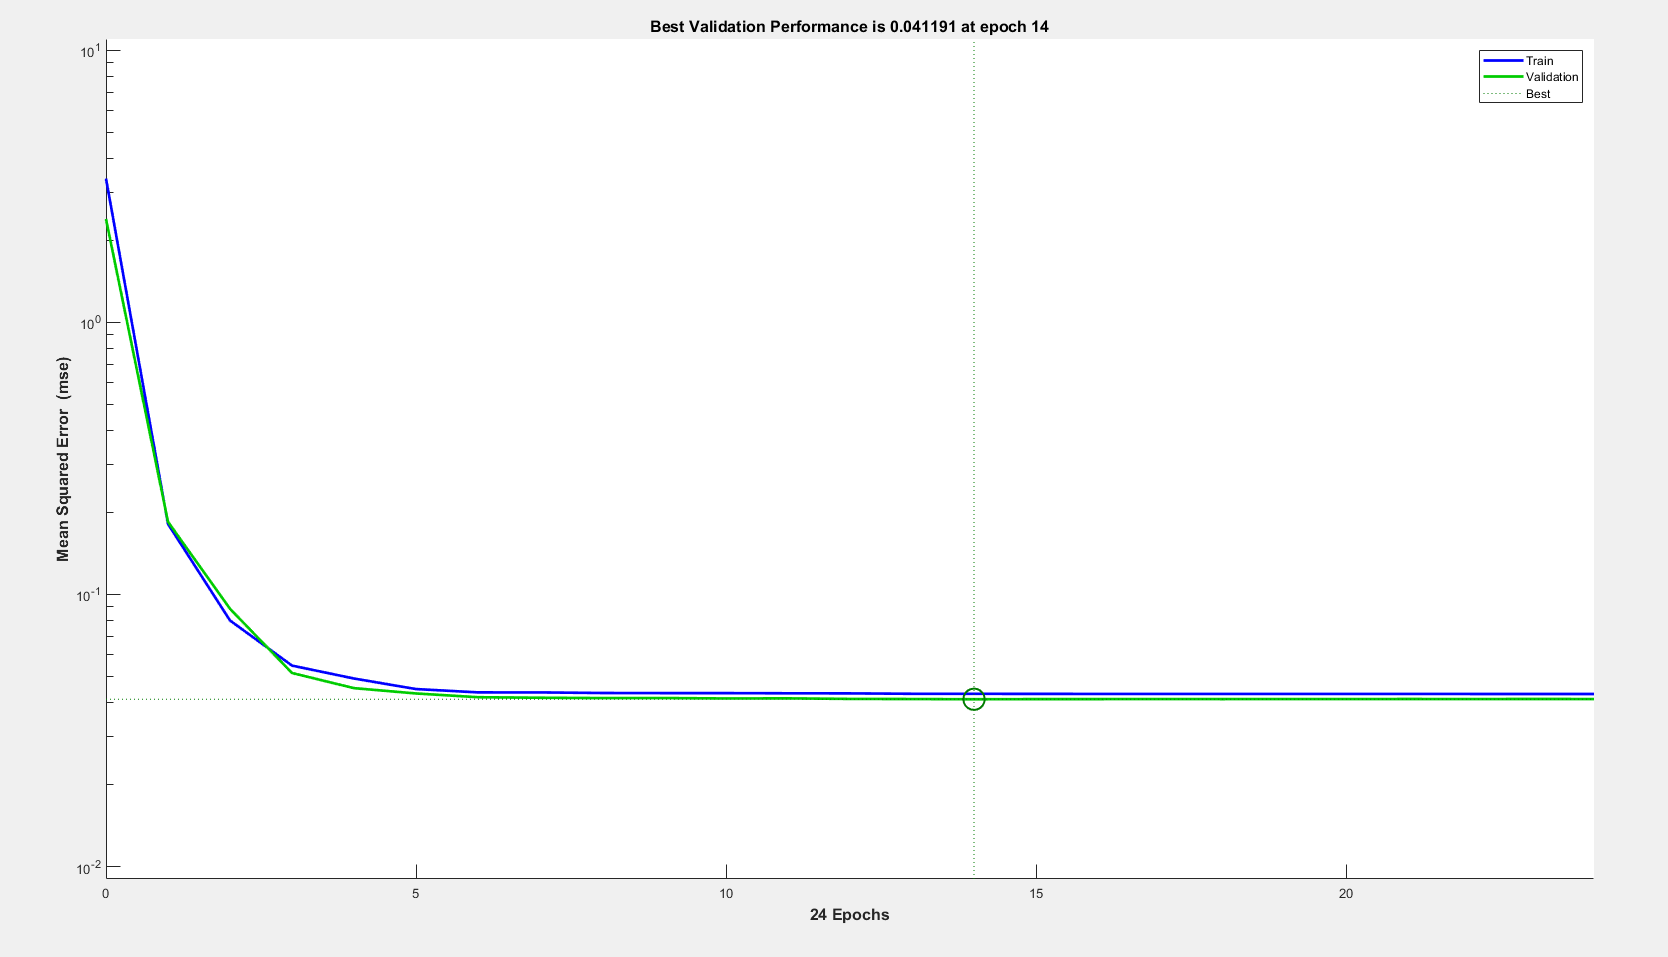
\includegraphics[width=\columnwidth]{imagens_windspeed/training_log_wind.png}
    \caption{Optimization curve showing the progression of training and validation errors.}
    \label{fig:wind_training_curve}
\end{figure}

The final assessment of the model's performance was conducted using a held-out test set comprising 104,854 independent samples. The resulting Mean Absolute Error (MAE) was $0.9669$ m/s. This value is highly significant, as it represents an average prediction error of less than 1 m/s in future wind speed, confirming the model's reliability for short-term meteorological forecasting.




\FloatBarrier
\subsection{Performance and Metrics (\textit{weatherHistory dataset})}
The hyperparameter optimization results for the weather station dataset, involving the prediction of apparent temperature, are presented in Table \ref{tab:weather_optimization}. Similar to the previous task, the grid search evaluated the impact of neuron count and activation functions over 30 independent trials per configuration.

\begin{table}[!htbp]
    \centering
    \caption{Neural Network Optimization Results for weatherHistory dataset}
    \label{tab:weather_optimization}
    \vspace{1em}
    \begin{tabular}{cccc}
        \toprule
        \textbf{Neurons} & \textbf{Activation} & \textbf{Mean Val MSE} & \textbf{Variance Val MSE} \\
        \midrule
        5  & "tansig" & 0.081584 & $4.7407 \times 10^{-4}$ \\
        5  & "poslin" & 0.086966 & $1.2022 \times 10^{-3}$ \\
        10 & "tansig" & 0.033847 & $3.8684 \times 10^{-5}$ \\
        10 & "poslin" & 0.022061 & $1.8038 \times 10^{-4}$ \\
        15 & "tansig" & 0.021651 & $1.8338 \times 10^{-5}$ \\
        15 & "poslin" & 0.018023 & $1.8953 \times 10^{-4}$ \\
        20 & "tansig" & 0.020038 & $3.4357 \times 10^{-5}$ \\
        \textbf{20} & \textbf{"poslin"} & \textbf{0.011805} & \boldmath{$9.4712 \times 10^{-5}$} \\
        \bottomrule
    \end{tabular}
    \par\vspace{1ex}
    \small \textbf{Note:} Highlighted row indicates the optimal configuration (20 neurons, \texttt{poslin}).
\end{table}

The empirical data demonstrates a clear correlation between network capacity and predictive accuracy. For this specific task, the \texttt{poslin} activation function coupled with 20 hidden neurons achieved the most significant error reduction, yielding a mean validation MSE of $0.011805$. This trend, visualized in Figure \ref{fig:weather_comparison_configs}, suggests that the additional neurons allowed the network to better map the complex interactions between temperature, humidity, and pressure that define the apparent temperature.

\begin{figure}[H]
    \centering
    
\includegraphics[width=\columnwidth]{imagens_weatherHistory/comparação estátistica dos erros das diferentes configs.png}
    \caption{Performance comparison of activation functions and hidden layer sizes for the weatherHistory dataset.}
    \label{fig:weather_comparison_configs}
\end{figure}

Following the identification of the optimal configuration, a final model was trained. The convergence behavior, shown in Figure \ref{fig:weather_training_curve}, reflects a stable optimization process with errors stabilizing at very low values.

\begin{figure}[H]
    \centering
    
\includegraphics[width=\columnwidth]{imagens_weatherHistory/validação.png}
    \caption{Training and validation error progression for the optimal weatherHistory model.}
    \label{fig:weather_training_curve}
\end{figure}

The final evaluation on the isolated test set yielded a Mean Absolute Error (MAE) of $0.0432$. This suggests that the engineered features, particularly the interaction between temperature and humidity, provided the network with sufficient information to reconstruct the apparent temperature formula with near-perfect accuracy.


\section{Discussion}
The results obtained across both regression tasks highlight the critical role of data preparation and feature engineering in the training of shallow neural networks. For the \textit{windSpeed} dataset, the challenge was primarily temporal and stochastic. By transforming the wind direction and timestamp into cyclic components and applying a logarithmic scaling to the wind speed, we were able to provide the network with a more stable and physically consistent input space. The final MAE of $0.9669$ m/s is a significant achievement for a single-minute forecast using a standard feedforward architecture, as it demonstrates that the network effectively captured the momentum and short-term trends of the wind.

In contrast, the \textit{weatherHistory} dataset presented a more deterministic problem. Apparent temperature is physically derived from current weather measurements, such as humidity and real temperature. This was reflected in the remarkably low MAE of $0.0432$. The high precision achieved here confirms that the engineered features, such as the heat index proxy and the wind chill effect, successfully exposed the underlying physical formulas to the network.

Across both datasets, the \texttt{poslin} (ReLU) activation function proved to be more efficient than the traditional \texttt{tansig}. This can be attributed to the fact that ReLU does not suffer from saturation for large positive values, which was particularly beneficial for handling the wide ranges of temperature and wind velocity. Furthermore, the low variance observed across the 30 independent training runs for each configuration validates the statistical significance of our hyperparameter selection and confirms that the models converged to stable, reproducible solutions.

\section{Conclusion}
This study successfully demonstrated the implementation of neural network-based regression for two distinct environmental forecasting problems. Through a rigorous methodology encompassing data cleaning, anomaly analysis, and specialized feature engineering, we transformed raw, sometimes inconsistent measurements into highly informative training sets.

The systematic hyperparameter grid search proved essential in identifying the optimal balance between network capacity and generalization. While shallow architectures were employed, the results show that when combined with robust pre-processing, these models are capable of achieving high predictive accuracy. Specifically, the wind speed forecast achieved an average error of less than 1 m/s, and the apparent temperature inference achieved near-formulaic precision.

In summary, the project confirms that the success of a neural network model is fundamentally tied to the precision of the data preparation and the clarity of its representation. The techniques refined throughout this study—most notably the trigonometric encoding of periodic variables and the strategic selection of non-linear transfer functions—establish a robust framework for addressing more complex meteorological forecasting and environmental regression challenges in the future.



\onecolumn
\appendix


\begin{lstlisting}[language=Matlab, caption={windspeed\_data\_cleaning.m}, captionpos=t]

\end{lstlisting}


\begin{lstlisting}[language=Matlab, caption={windspeed\_data\_visualization.m}, captionpos=t]

\end{lstlisting}


\begin{lstlisting}[language=Matlab, caption={windspeed\_model\_training.m}, captionpos=t]

\end{lstlisting}


\begin{lstlisting}[language=Matlab, caption={weatherStation\_model\_training.m}, captionpos=t]

\end{lstlisting}
\end{document}